% !TEX root = main.tex
\section{Dynamics}
A train traversing a railway bridge creates actions in longitudinal, lateral, and vertical directions. Braking and traction from a passing train causes longitudinal forces
Rocking, or rotations around an axis parallel to the longitudinal axis of the bridge, and vertical dynamic forces are created by structure-track-vehicle conditions and interactions.
\subsection{Rocking and vertical dynamic forces}
Lateral rocking of moving vehicles provide amplification of vertical  wheel loads. This amplification increases the stresses in the members supporting the track.

Superstructure-vehicle interaction creates a vertical dynamic amplification of moving loads, which will result in vibrations causing additional stresses in members supporting the track.

The unloaded simply supported beam frequency $\omega_1 = \frac{\pi^2}{L^2}\sqrt{\frac{EI}{m}}$, provides a basic indicator of superstructure vertical dynamic response.

\section{Trains}
\subsection{NSB92}
\label{appendix:nsb92}
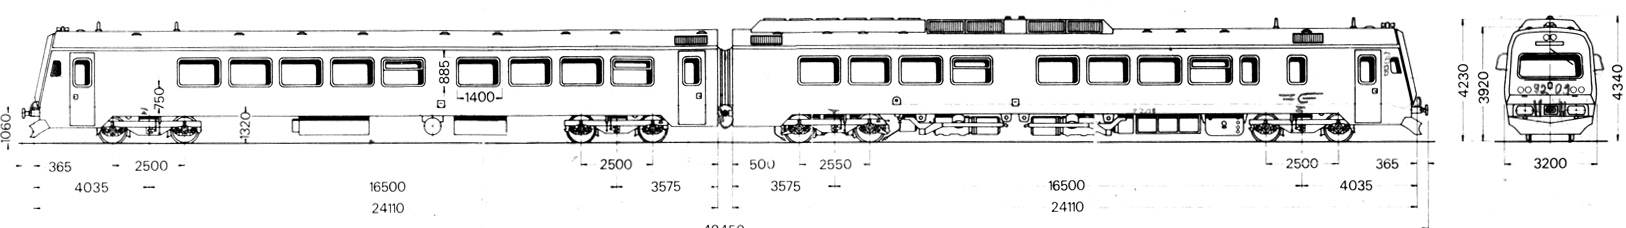
\includegraphics[width=0.8\pageheight, height=0.5\pagewidth, angle=270]{./figures/nsb92.png}
\subsection{Freight train}
